\capitulo{5}{Aspectos relevantes del desarrollo del proyecto}

\section{Entorno de desarrollo}
Como entorno de desarrollo de los prototipos hemos designado Jupyter ya que en sus notebooks interactivos puedes ejecutar directamente código Python como si fuese un interprete.

\subsection{Ventajas}
\begin{itemize}
\item He podido añadir widgets para calibrar en buen grado las funciones que hemos utilizado.\\
Gracias a estos widgets podemos dar valores e ir viendo como cambia la salida de la función de forma interactiva.\ref{fig:5.1}

\begin{figure}[h]
\centering
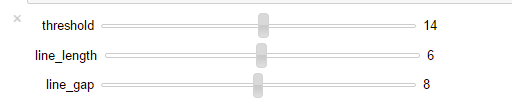
\includegraphics[width=0.65\textwidth]{Widget}
\caption{Ejemplo de un widget sobre la función de hough}
\label{fig:5.1}
\end{figure}

\item Su rápida visualización sin tener grandes conocimientos de interfaz gráfica ha sido un gran apoyo para poder visualizar desde el principio las imágenes procesadas y como quedaban.\ref{fig:5.2} 

\begin{figure}
\begin{subfigure}[b]{.5\linewidth}
\centering\large 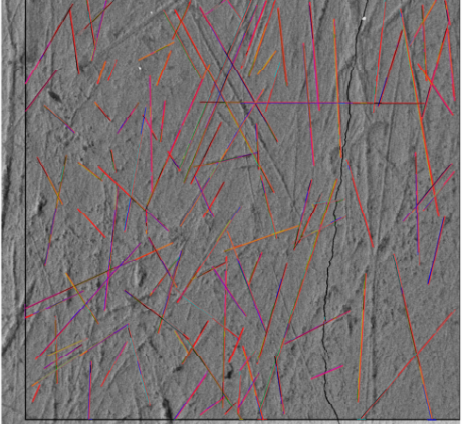
\includegraphics[width=.9\textwidth]{ComparativaLineas2}
\caption{Lineas antes de unir}
\end{subfigure}%
\begin{subfigure}[b]{.5\linewidth}
\centering\large 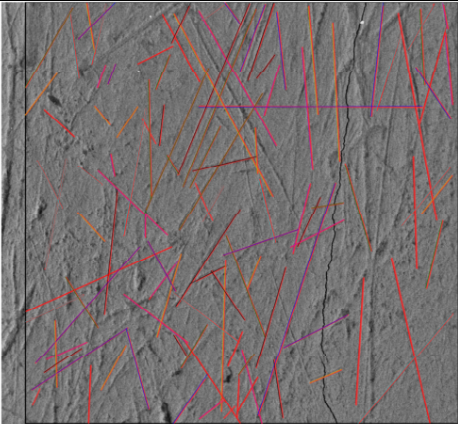
\includegraphics[width=.9\textwidth]{ComparativaLineas1}
\caption{Lineas después de unir}
\end{subfigure}
\caption{Ejemplo de una visualización del resultado intermedio de las funciones.}\label{fig:5.2}
\end{figure}


\item Desde el propio entorno puedes ejecutar no solo código estructurado en script sino también código estructurado en clases y llamadas a métodos es como un IDE pero con limitaciones.\ref{fig:5.3}

\begin{figure}[h]
\centering
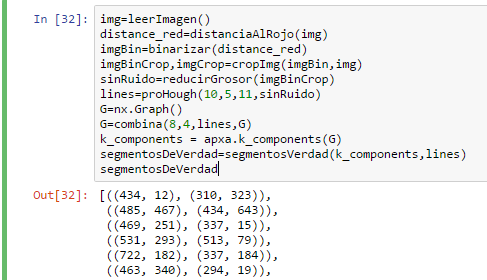
\includegraphics[width=0.65\textwidth]{Ejecucion}
\caption{Ejemplo de una Ejecución.}
\label{fig:5.3}
\end{figure}

\item Multitud de librerías y funciones que en entornos parecidos como matlab serian de pago y aquí al ser software libre el ejemplo anterior lo resume en una librería numpy \cite{Numpy}.
\end{itemize}

\section{Procesado imagen}
Para llegar a conseguir calcular las lineas que había pintadas en las imágenes tube que realizar una serie de pasos que vamos a resumir en tres etapas.
\subsection{Binarización}
Partiendo de una imagen que solo tenia lineas en rojo pintadas encima de las estrías producidas por el desgaste y lo demás de la imagen en escala de grises, lo primero fue leer la imagen a trabes de las funciones ya programadas en la librería de Scikit-Image(skimage).\\
Una vez que tenemos la imagen guardada en el espacio de color RGB podemos empezar el procesado quedándonos con el canal Rojo.\\
Calculamos la distancia de cada pixel de la imagen al color rojo restando, uno menos el valor absoluto del pixel en el canal S (saturación) del espacio de color HSV , (restando el valor absoluto a la unidad conseguimos normalizar entre [0-1])y pasamos la imagen de distancias a blanco y negro y así tendremos un valor entre 0 y 256 en cada pixel correspondiente a la distancia al rojo cuanto mas alejado mas negro y los que sean rojos en blanco.\\
Para que la diferencia sea blanco o negro binarizamos la imagen con un valor umbral calculado como threshold otsu y así la imagen los valores de la distancia que sean mayores que el umbral pasaran a valer máximo y los que no consigan pasar el umbral serán los bordes(blanco).\ref{fig:5.4}


\begin{figure}
\begin{subfigure}[c]{.5\linewidth}
\centering\large 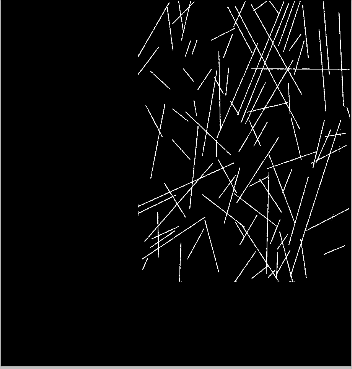
\includegraphics[width=.9\textwidth]{paso1Binariza}
\caption{Original}
\end{subfigure}%
\begin{subfigure}[c]{.5\linewidth}
\centering\large 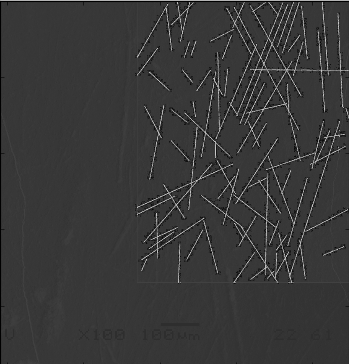
\includegraphics[width=.9\textwidth]{paso1DistanciaR}
\caption{Distancia al rojo}
\end{subfigure}
\begin{subfigure}[c]{.5\linewidth}
\centering\large 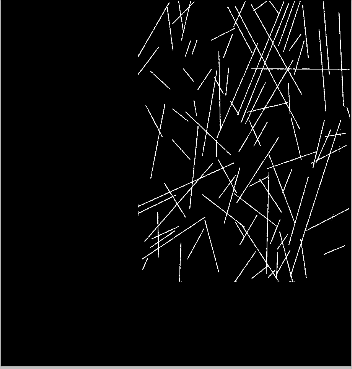
\includegraphics[width=.9\textwidth]{paso1Binariza}
\caption{Imagen binarizada}
\end{subfigure}
\caption{Resumen visual binarización.}\label{fig:5.4}
\end{figure}


\subsection{Obtener segmentos}
Partimos de la imagen binarizada y lo primero es reducir el grosor de las lineas detectadas a un pixel eso lo conseguimos llamando a la función skeletonize que nos devuelve la imagen con las lineas de un pixel (así no acumulamos errores y es mas rápida la búsqueda de rectas).\\
Seguidamente llamamos a la función "probabilistic hough line" que nos va a encontrar segmentos que formaran las lineas el funcionamiento ha sido explicado en el apartado (conceptos teóricos).\ref{fig:5.5}


\begin{figure}
\begin{subfigure}[c]{.5\linewidth}
\centering\large 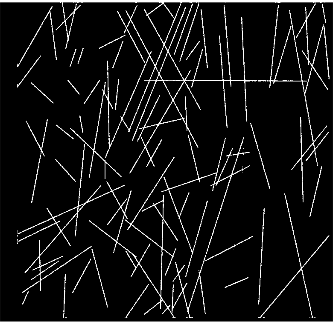
\includegraphics[width=.9\textwidth]{paso2Binaria}
\caption{Binarizada}
\end{subfigure}%
\begin{subfigure}[c]{.5\linewidth}
\centering\large 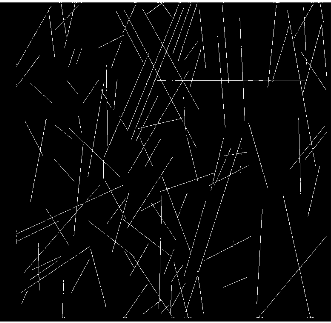
\includegraphics[width=.9\textwidth]{Paso2Skele}
\caption{Lineas a 1 pixel}
\end{subfigure}
\begin{subfigure}[c]{.5\linewidth}
\centering\large 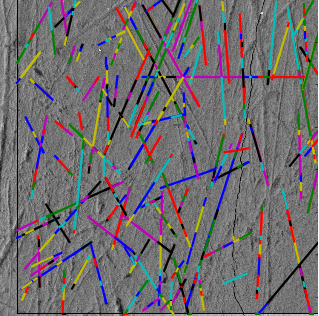
\includegraphics[width=.9\textwidth]{Paso2Segmentos}
\caption{Imagen original con segmentos}
\end{subfigure}
\caption{Resumen visual Obtener Segmentos.}\label{fig:5.5}
\end{figure}

\subsection{Procesado de segmentos}
Llegados a este punto lo que tenemos son muchos segmentos que forman las lineas reales y tenemos que unirlos.\\
Para ello vamos a usar la teoría de grafos añadiendo los segmentos a un grafo.\\
Para unir dos segmentos tiene que cumplirse que la distancia mínima entre sus extremos sea menor que un umbral y si pasa este punto comprobaremos que el angulo que forman entre ellas sea menor a otro umbral y si cumplen las dos condiciones añadiremos un camino al grafo desde la recta uno a la recta dos.\ref{fig:5.6}



\begin{figure}
\begin{subfigure}[b]{.5\linewidth}
\centering\large 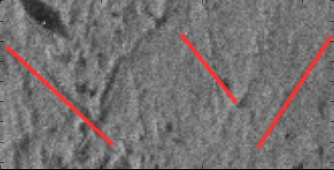
\includegraphics[width=.9\textwidth]{grafoLineasOri}
\caption{Imagen con segmentos en rojo.}
\end{subfigure}
\begin{subfigure}[b]{.5\linewidth}
\centering\large 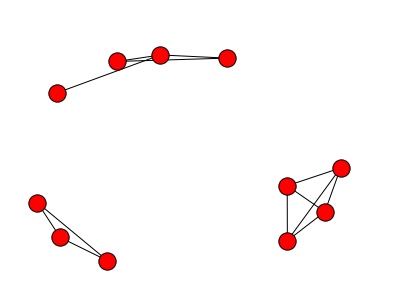
\includegraphics[width=.9\textwidth]{grafo}
\caption{Grafo de clusters de segmentos.}
\end{subfigure}
\caption{Resumen visual procesado de Segmentos.}\label{fig:5.6}
\end{figure}

\subsection{Recuperación de lineas}
Ahora lo que tenemos es un grafo con clusters ya que cada cluster se identifica con únicamente una recta y tendremos tantos como rectas.
Un problema de grafos es el problema de las k-componentes pero a nosotros solo nos interesan las 1-componentes del grafo ya que cada grupo de estos segmentos "cercanos" se corresponde con una recta real.
devolvemos la combinación de los segmentos mas relevantes de cada cluster y estos se convierten en nuestra buscada linea real.\ref{fig:5.7}
\begin{figure}[h]
\centering
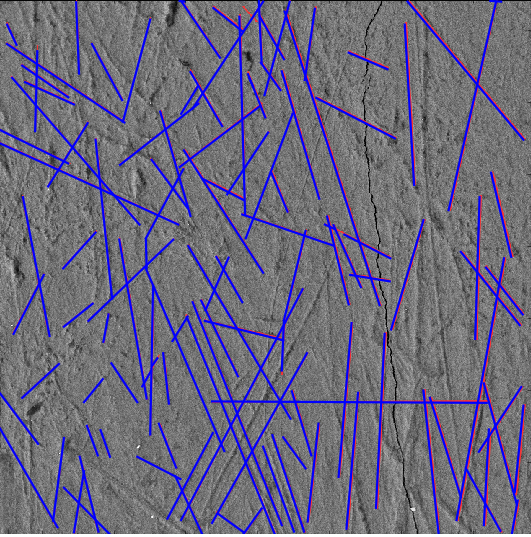
\includegraphics[width=0.65\textwidth]{ResultanteDelGrafo}
\caption{Lineas obtenidas después de procesar el grafo}
\label{fig:5.7}
\end{figure}

\subsection{Resumen pasos}

\begin{itemize}
\item Binarizar la imagen para solo quedarnos con los objetos de interés
\item Obtener segmentos que forman trozos de las lineas.
\item Añadir caminos entre las lineas cercanas en un grafo
\item obtener los grupos de lineas próximas y devolver la recta que las una. 
\end{itemize}

\section{Interfaz}
\subsection{Primera versión}

Para el desarrollo de la interfaz gráfica pensé en una una planificación espacial acorde con los elementos que esta contendría por lo que un layout que seria muy adecuado podría ser un border layout pero como no existe en PyQt4 lo he tenido que simular gracias a apilar layouts de otros tipos y consiguiendo tener una botonería arriba del todo y dos columnas debajo claramente diferenciadas en la que en una estuviera la imagen que vamos a mostrar y en la otra las funcionalidades.\ref{fig:5.8}

\begin{figure}[h]
\centering
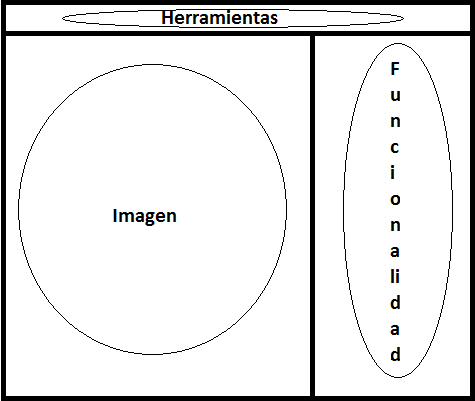
\includegraphics[width=0.65\textwidth]{disenoInter}
\caption{Diseño de la interfaz de usuario}
\label{fig:5.8}
\end{figure}

\subsection{Versión a evaluar}

En otro Sprint del proyecto lo que he usado han sido pestañas para así tener en la zona de funcionalidades los modos de trabajo de la aplicación claramente separados.\ref{fig:5.9}

\begin{itemize}
\item El modo uno.
\item El modo dos.
\item El modo tres.
\end{itemize}


\begin{figure}[h]
\centering
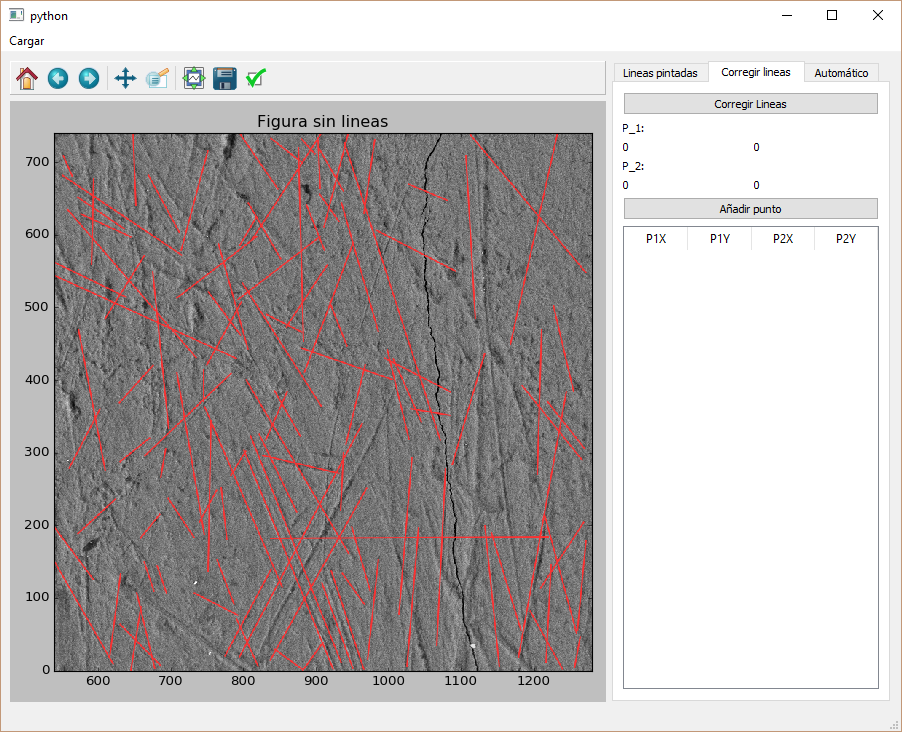
\includegraphics[width=0.65\textwidth]{disenoWi}
\caption{Diseño de la interfaz de usuario}
\label{fig:5.9}
\end{figure}
\subsubsection{Barra de herramientas}
Es una sección de la interfaz que nos va permitir de momento la carga de imágenes para su procesado (También funciona con Ctrl+O).\ref{fig:5.10}
\begin{figure}[h]
\centering
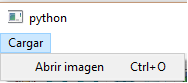
\includegraphics[width=0.65\textwidth]{BarraHerramientas}
\caption{Barra de herramientas de la aplicación}
\label{fig:5.10}
\end{figure}

\subsubsection{Barra de herramientas de la imagen}
Es una sección de la interfaz que nos permitirá manipular la imagen para realizar estas acciones:\ref{fig:5.11}

\begin{itemize}
\item Volver al principio. 
\item Retroceder un paso.
\item Avanzar un paso.
\item Desplazar la imagen.
\item Aumentar la región que seleccionemos.
\item Configurar la región, bordes, etc.
\item Guardar la imagen con su escala.
\item configurar el tamaño y numeración de los ejes.
\item Coordenadas actuales del ratón.
\item Niveles de color de los canales R G B del espacio RGB.
\end{itemize}

\begin{figure}[h]
\centering
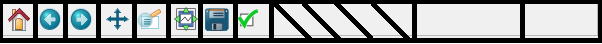
\includegraphics[width=0.95\textwidth]{toolbar}
\caption{Barra de herramientas de la imagen}\label{fig:5.11}
\end{figure}


\subsubsection{FigureCanvas de la imagen}
Es la región donde se muestra la imagen que va a ser ligeramente mas grande que la parte de las pestañas.\ref{fig:5.12}
\begin{figure}[h]
\centering
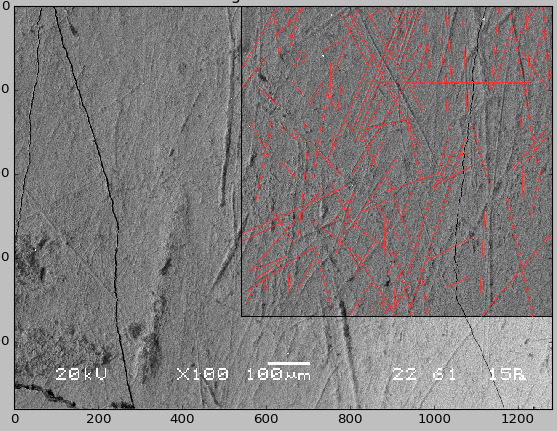
\includegraphics[width=0.65\textwidth]{FigureCanvas}
\caption{FigureCanvas de la imagen}
\label{fig:5.12}
\end{figure}


\subsubsection{Pestañas}
Sección de la imagen donde estarán implementadas las funcionalidades para visualizar las lineas que son detectadas por el algoritmo en la imagen.\ref{fig:5.13}
\begin{itemize}
\item El modo primero es la detección de los surcos en rojo en los dientes 
\item El modo segundo es la corrección/detección manual de las lineas por una persona y quedando reflejadas en la imagen.
\item El modo tercero es la ultima parte del proyecto que consistirá en hacer todo el proceso anterior de forma automática.
\end{itemize}

\begin{figure}[h]
\centering
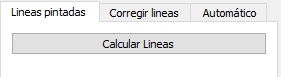
\includegraphics[width=0.65\textwidth]{Pestanas}
\caption{Pestañas}
\label{fig:5.13}
\end{figure}

